\subsection{Tiempo de uso promedio de los usuarios}

Los datos obtenidos de MiBici contienen el tiempo inicial y final del uso de una bicicleta durante su uso. En base a este tiempo calculado en minutos, se usaron las ecuaciones \ref{eq:monthly_hourly_mean}, \ref{eq:monthly_hourly_var}, \ref{eq:daily_hourly_mean} y \ref{eq:daily_hourly_var}. Los resultados obtenidos son los siguientes:

\subsubsection{Promedio y desviación estandar mensual por hora}

En la figura \ref{fig:monthly_hourly_mean_time} se visualiza que existe un aumento en el tiempo de uso entre los meses octubre y diciembre. Este último coincide con el fin de la temporada con más frecuencia de lluvias y una disminución de la temperatura\cite{clima_guadalajara}. En la misma figura se presenta un mínimo entre los meses de mayo y agosto. Con ayuda de la figura \ref{fig:monthly_hourly_var_time} se obtiene que el tiempo de uso de los usuarios entre los meses de octubre y diciembre tienen una mayor variación y esto puede deberse a que la baja temperatura y baja probabilidad de lluvia\cite{clima_guadalajara}. Ya que los usuarios pueden sentir menos preocupación de las vías públicas y el usar la bicicleta representa más un momento de descanso que estar alerta de su alrededor.

\begin{figure}[H]
    \centering
    \begin{subfigure}[b]{8cm}
        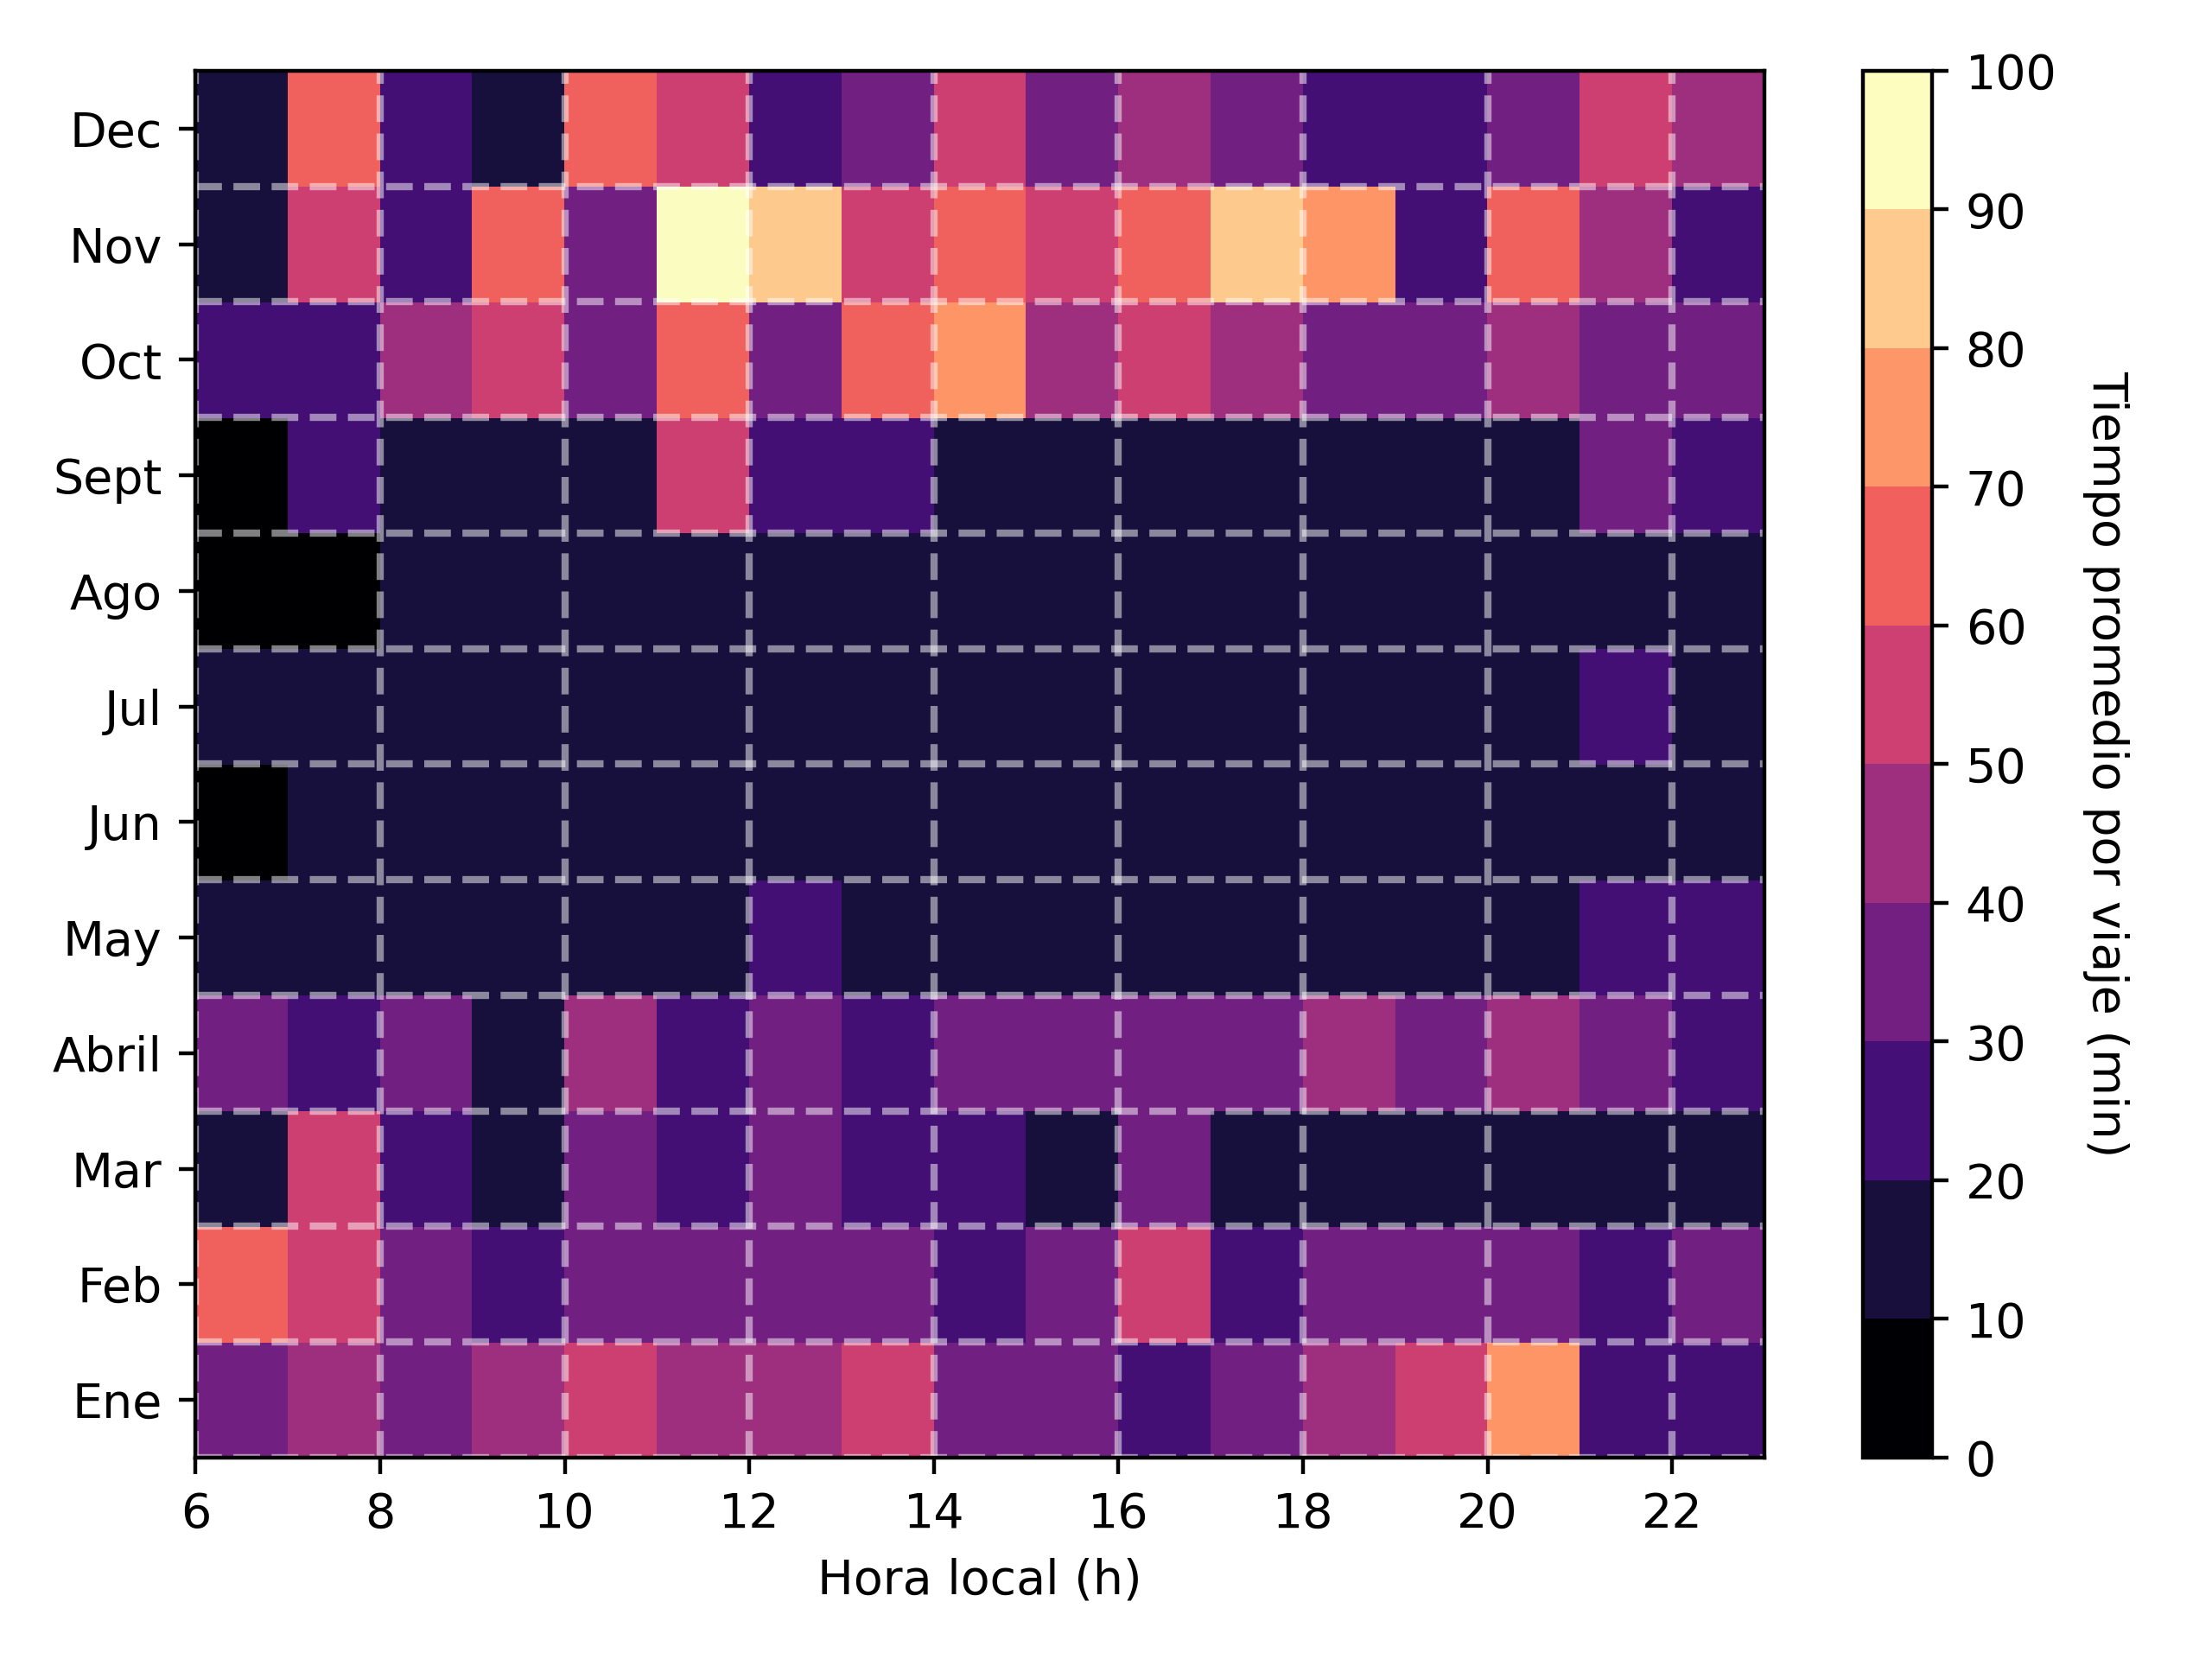
\includegraphics[width=8cm]{Graphics/monthly_hourly_mean_time_travel.png}
        \caption{Promedio mensual del tiempo de uso.}
        \label{fig:monthly_hourly_mean_time}
    \end{subfigure}
    \begin{subfigure}[b]{8cm}
        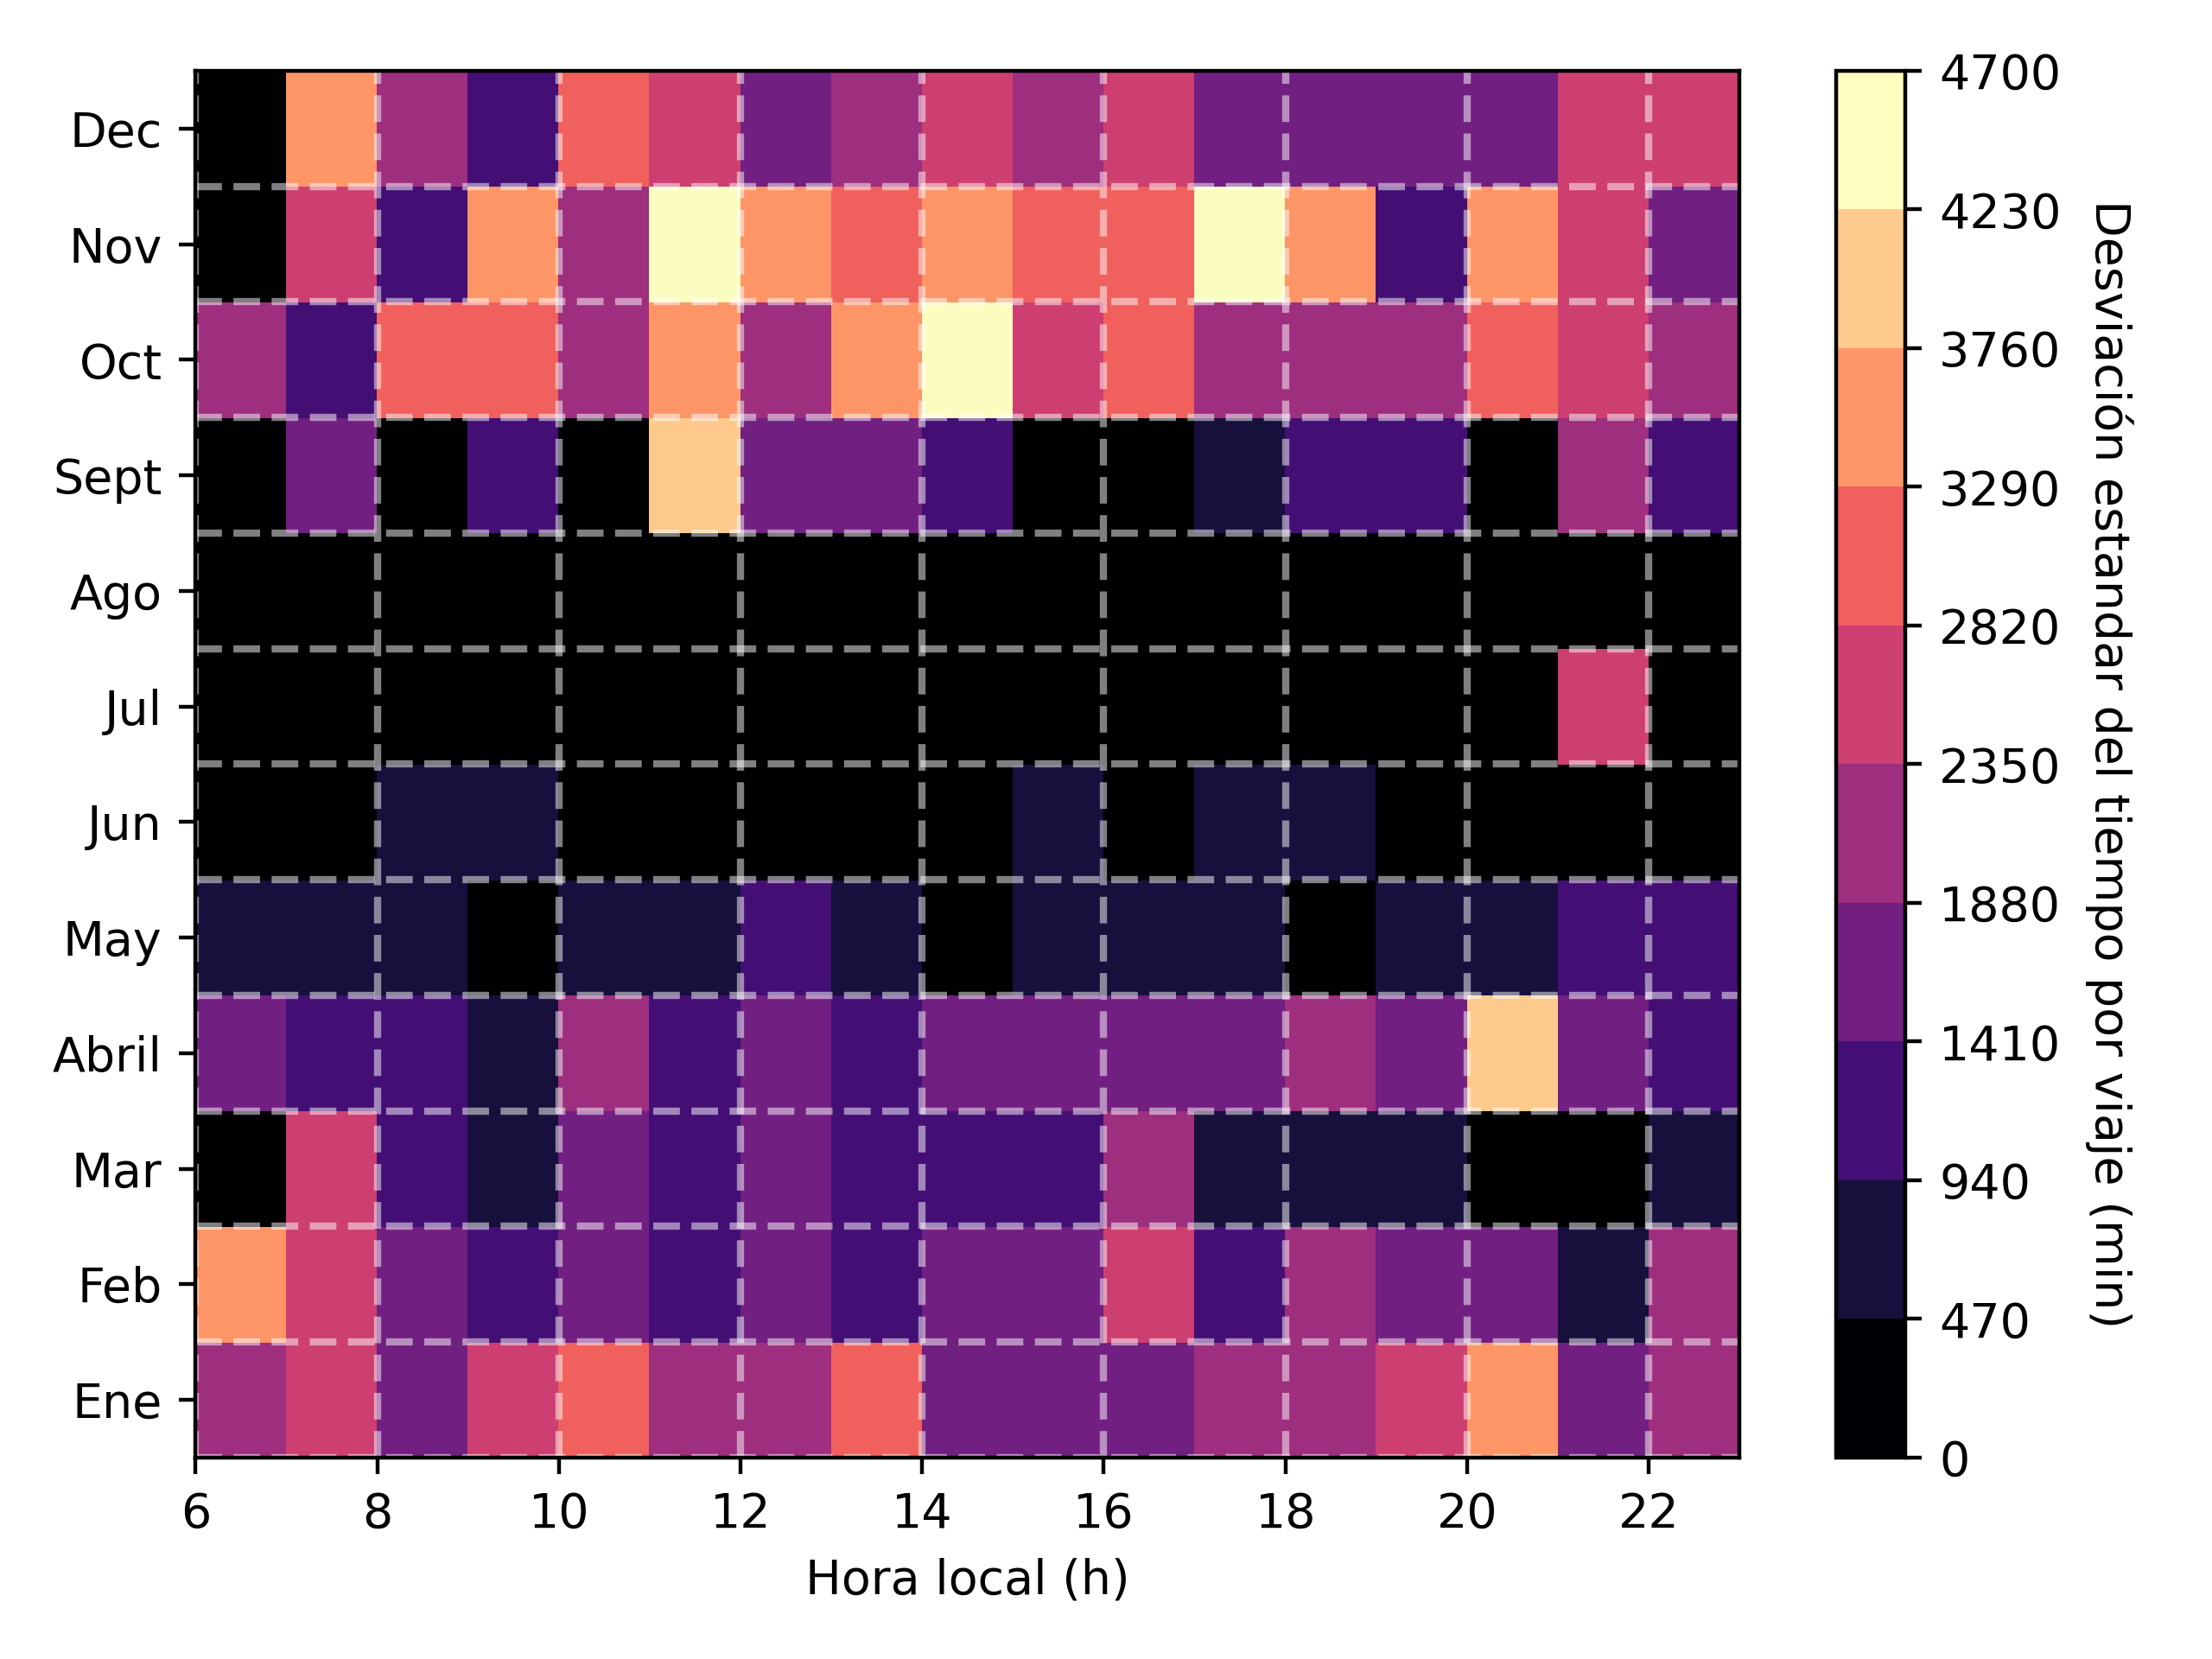
\includegraphics[width=8cm]{Graphics/monthly_hourly_var_time_travel.png}
        \caption{Desviación estandar del tiempo de uso.}
        \label{fig:monthly_hourly_var_time}
    \end{subfigure}
    \caption{Tiempo de uso promedio y desviación estandar mensual por hora de lo usuarios calculadas con las ecuaciones \ref{eq:monthly_hourly_mean} y \ref{eq:monthly_hourly_var}.}
    \label{fig:monthly_hourly_time}
\end{figure}

\subsubsection{Promedio y desviación estandar diaria semanal por hora}

En la figura \ref{fig:daily_hourly_time} se aprecia que no hay alguna preferencia en los tiempos de uso en los dias entre semana, por lo que se podria estimar un tiempo promedio por día para toda la semana. Con esto el factor más importante a tomar en cuenta es el mes del que se trate, ya que como se describió en la figura \ref{fig:monthly_hourly_time}, sí existen variaciones a lo largo del año. En la figura \ref{fig:daily_hourly_var_time} entre las 8 y 10 am se ve que existe una mayor variación en el tiempo de uso. Lo cual concuerda con lo antes mencionado en la figura \ref{fig:daily_hourly_var_distance}

\begin{figure}[H]
    \centering
    \begin{subfigure}[b]{8cm}
        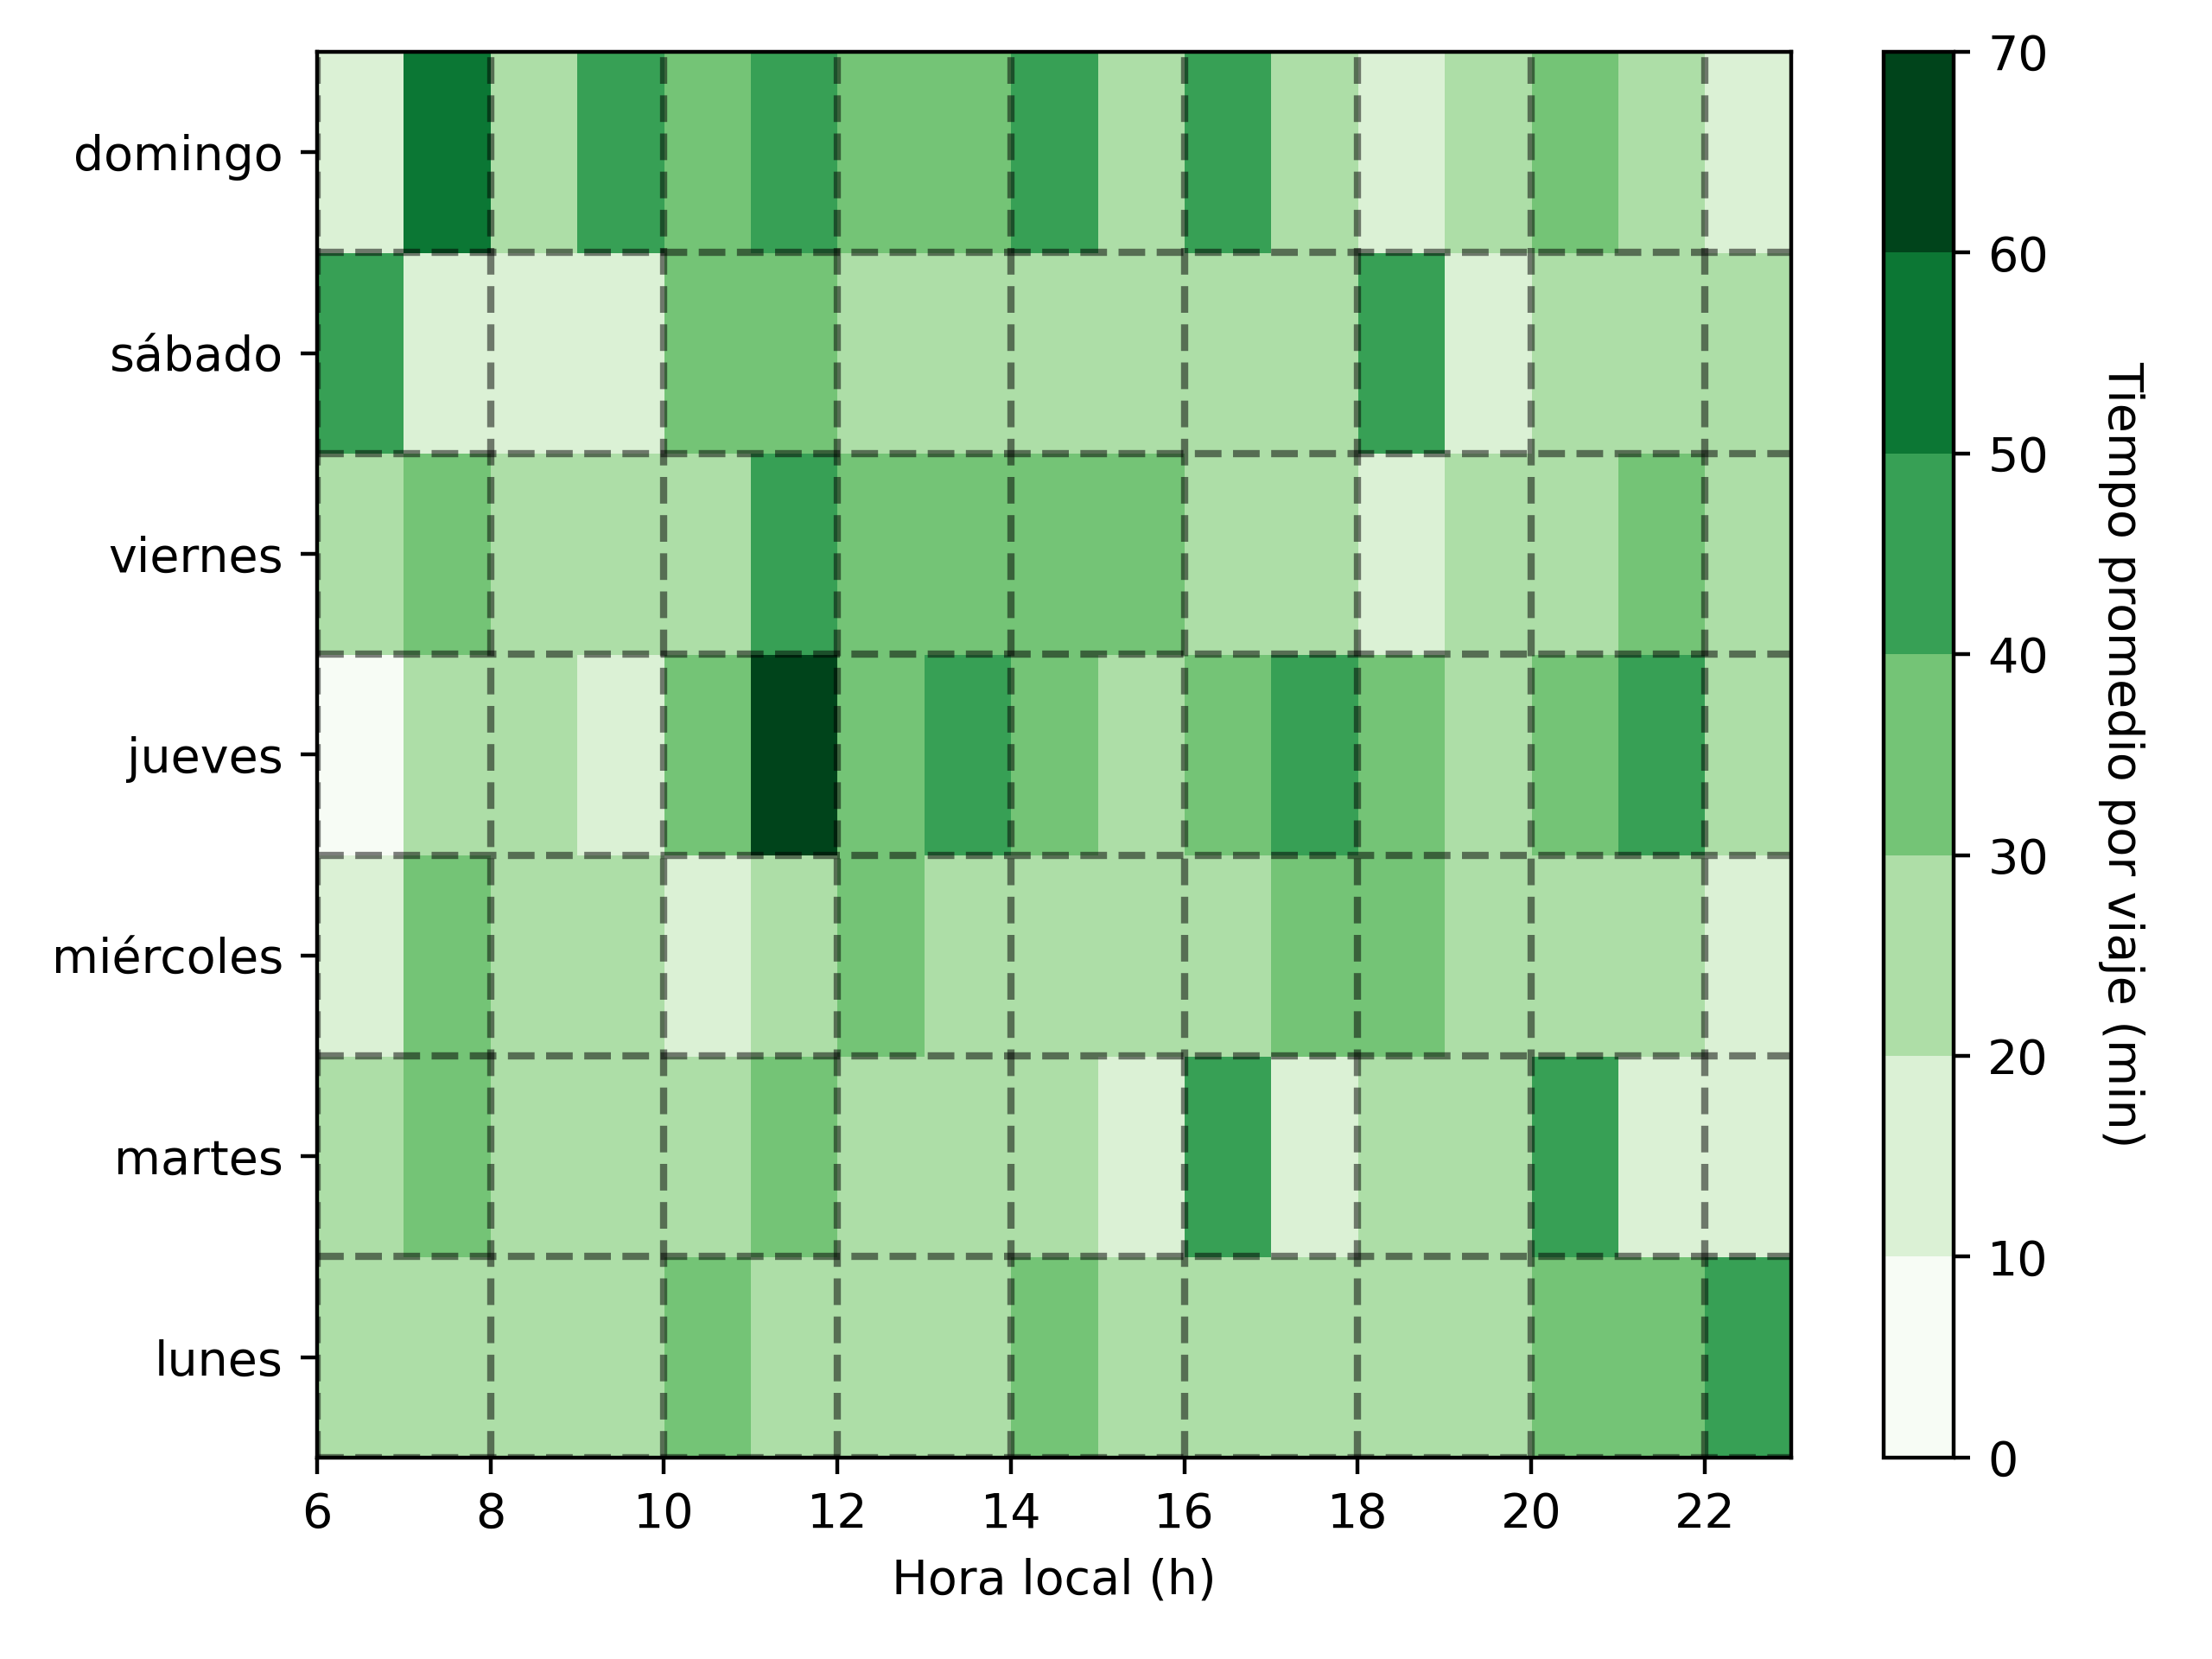
\includegraphics[width=8cm]{Graphics/daily_hourly_mean_time_travel.png}
        \caption{Promedio diario semanal.}
        \label{fig:daily_hourly_mean_time}
    \end{subfigure}
    \begin{subfigure}[b]{8cm}
        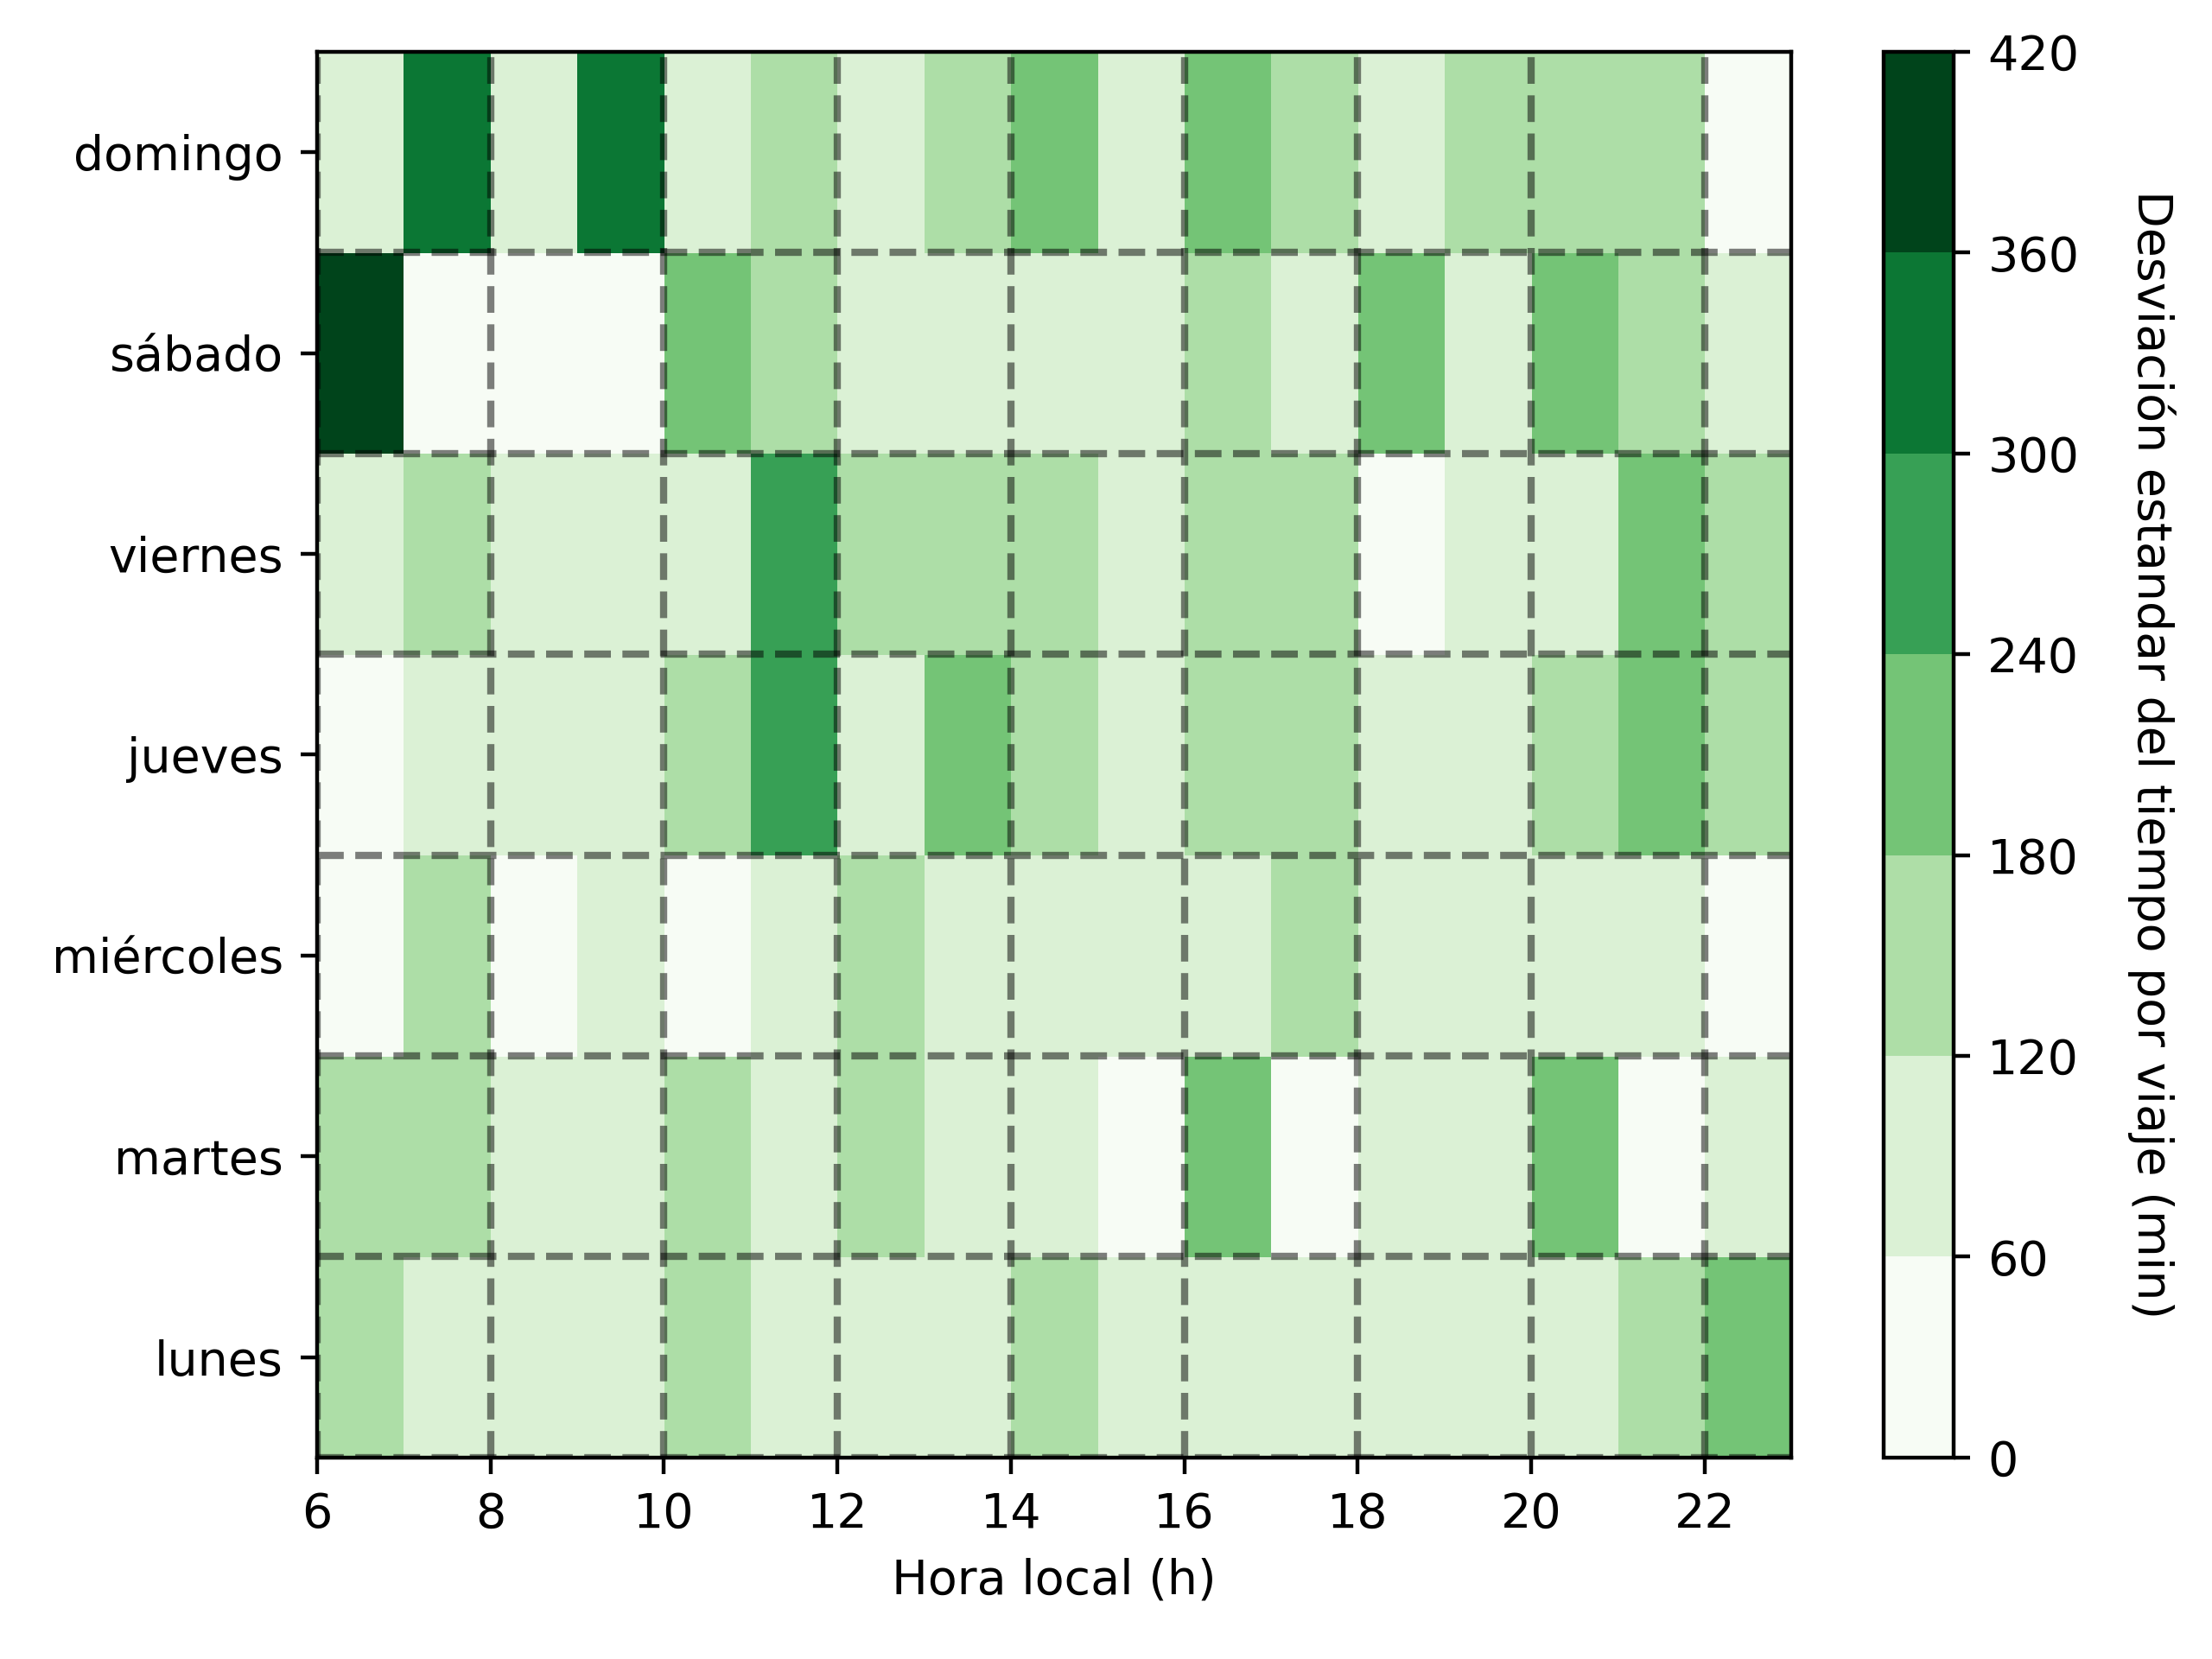
\includegraphics[width=8cm]{Graphics/daily_hourly_var_time_travel.png}
        \caption{Desviación estandar diaria semanal.}
        \label{fig:daily_hourly_var_time}
    \end{subfigure}
    \caption{Tiempo de uso promedio y desviación estandar diaria semanal por hora de los usuarios calculadas con las ecuaciones \ref{eq:daily_hourly_mean} y \ref{eq:daily_hourly_var}.}
    \label{fig:daily_hourly_time}
\end{figure}
